%Positionierung dieses Tikz-Pictures anpassen, da die Stützpunkte des geekrümmten Pfeils außerhalb der tatsächlichen Boundingbox liegen und diese mitzählen.
\vspace*{-1cm} 
\begin{adjustbox}{width=0.9\textwidth}
	\begin{tikzpicture}[every node/.style={inner sep=0,outer sep=0}]
	
		%Bild der Oberfläche laden
		\node [anchor=north] (imgOberflaeche) at (0,0) {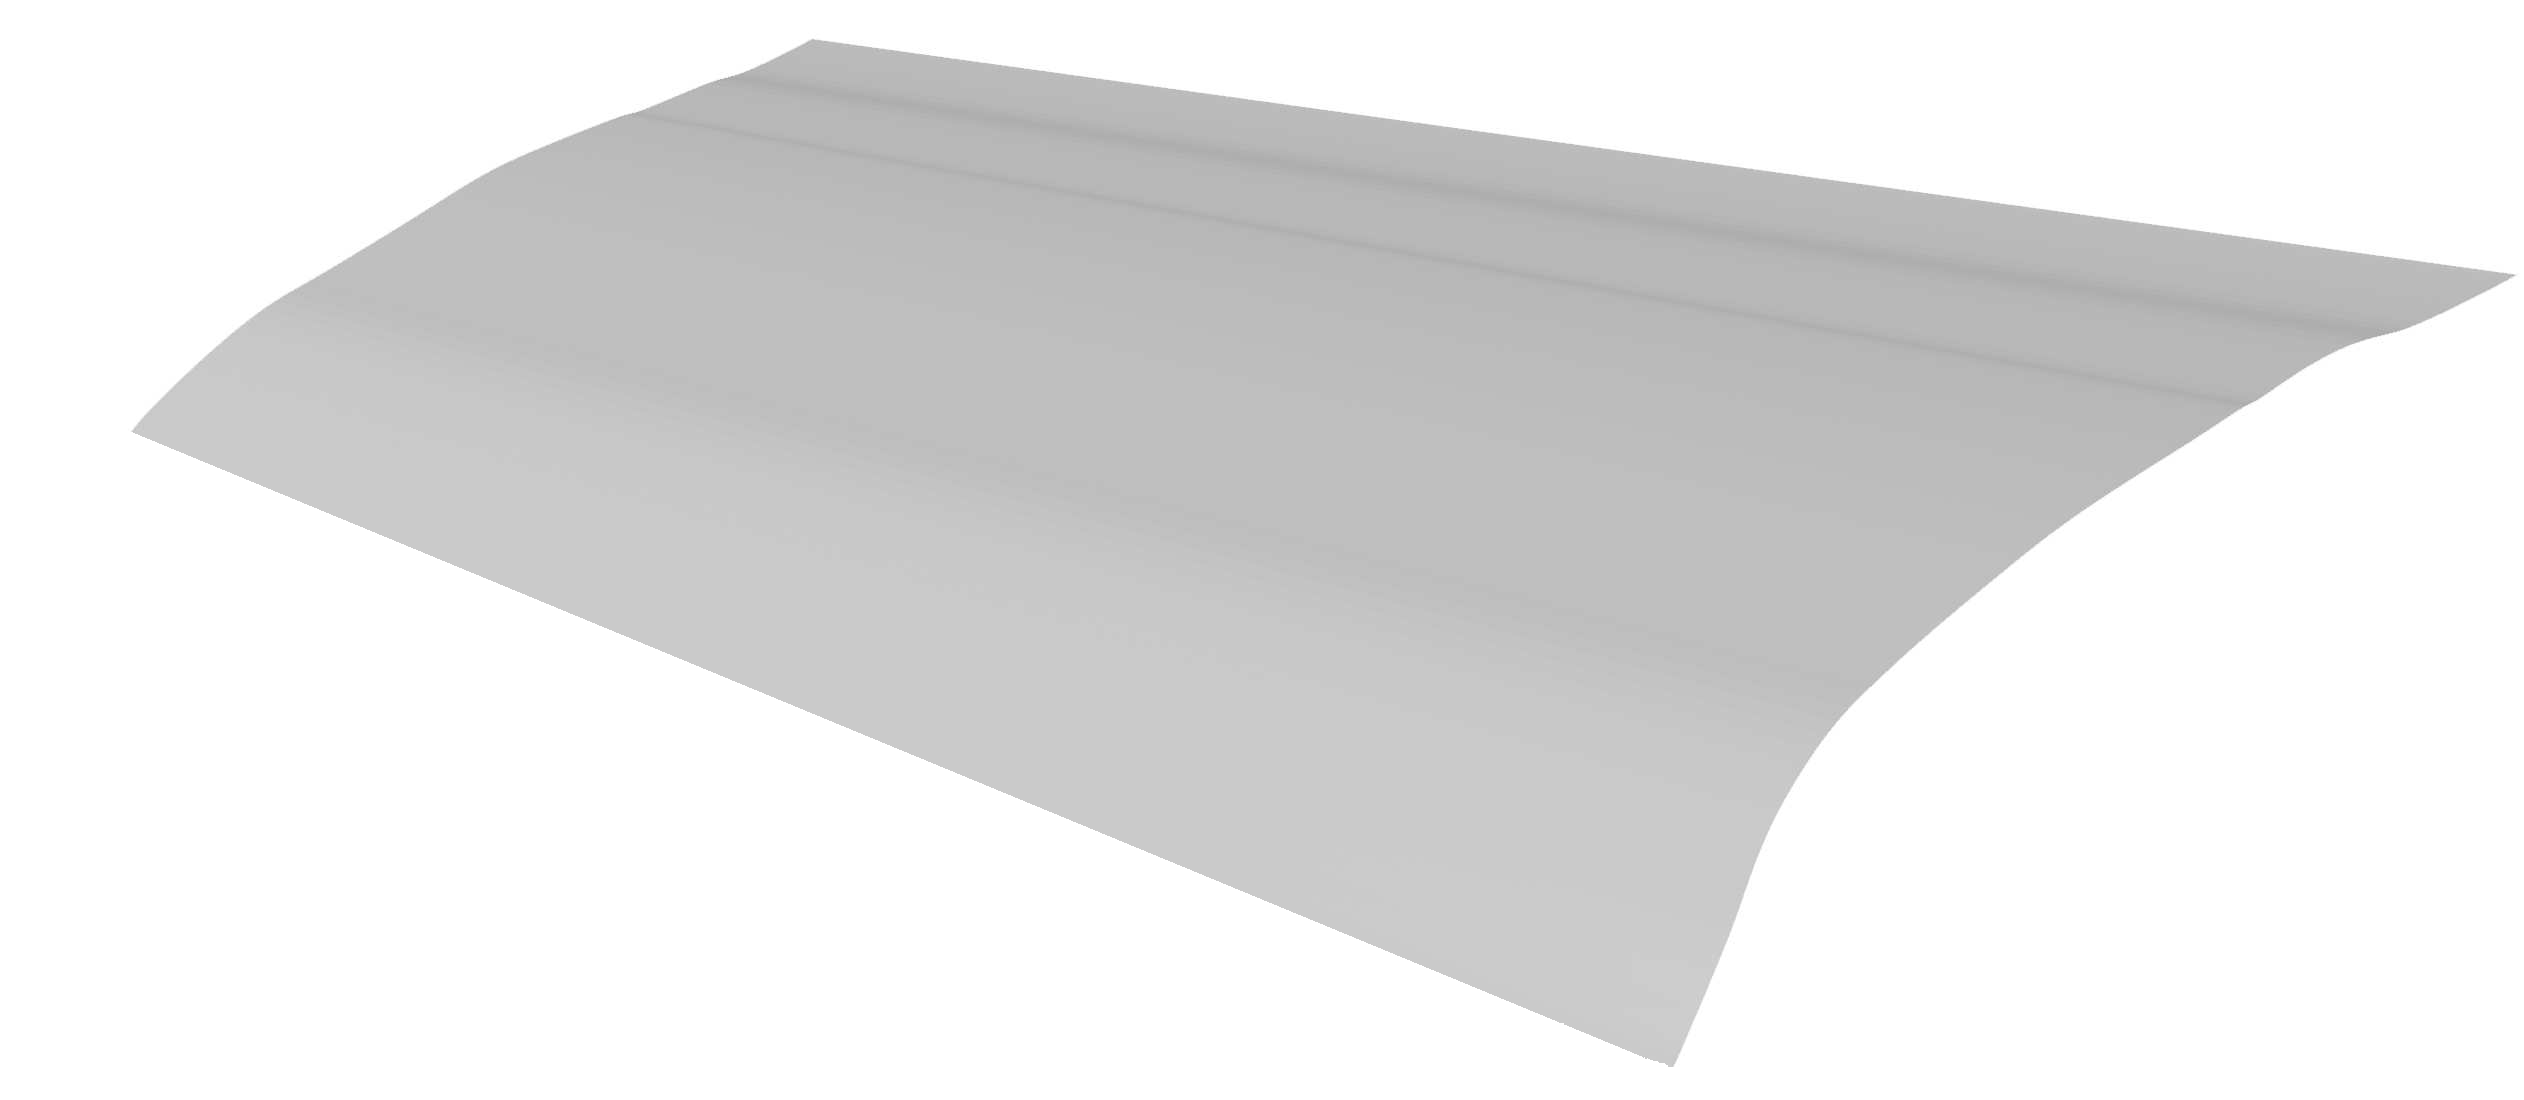
\includegraphics[width=360pt]{04_deflektometrischeRegistrierung/figures/oberflaeche}};
		
		%Punkte setzen
		\node (monitorpunkt) at (-6,0) {};
		\node (objektpunkt) at (0,-3) {};
		\node (kamerapunkt) at (4,1.5) {};
		
		%Kamera und Monitor zeichnen
		\node [trapezium, draw, minimum width=1.5cm, minimum height=1cm, trapezium left angle=120, trapezium right angle=60, trapezium stretches=false, inner sep=2] (kamera) at (kamerapunkt) {};
		\node [trapezium, draw, rotate=35, minimum width=1cm, minimum height=1.5cm, trapezium left angle=40, trapezium right angle=140, trapezium stretches=false, inner sep=2, fill=black!5] (monitor) at (monitorpunkt) {};		
		
		%Punkte beschriften
		\node [circle,fill=black,minimum size=5pt] at (monitorpunkt) {};
		\node [circle,fill=black,minimum size=5pt] at (objektpunkt) {};
		\node [circle,fill=black,minimum size=5pt] at (kamerapunkt) {};
		\node [below left=4pt and 2pt of monitorpunkt] {\Large M};
		\node [below=6pt of objektpunkt] {\Large P};
		\node [below right=1pt and 5pt of kamerapunkt] {\Large K};
		
		%Lichtstrahl zeichnen
		\draw[red,very thick,midarrow] (monitorpunkt) -> (objektpunkt);
		\draw[red,very thick,midarrow] (objektpunkt) -> (kamerapunkt);
		
		%Abbildung zeichnen
		\draw[Green,very thick,-{Latex[width=3mm]}] (kamerapunkt) to [out=120, in=60] node[midway,outer sep=4pt,above] {\Large \acrshort{lr}} (monitorpunkt);

		%Oberflächennormale zeichnen
		\draw[very thick,-{Latex[width=3mm]}] (objektpunkt) --++ (100.5:1.5cm) node[right=5pt] {\Large $n$};
		%Monitor, Oberfläche und Kamera beschriften
		\node[anchor=east] at (-5.5,1.7) {\Large Bildschirm};
		\node[anchor=west] at (3.9,0.6) {\Large Kamerasensor};
		\node[anchor=west] at (3.2,-4.1) {\Large Oberfläche};
		
	\end{tikzpicture}
\end{adjustbox}
\caption[Abbildungssystem einer spiegelnden Oberfläche]{Abbildungssystem einer spiegelnden Oberfläche. M $\subset L$ entspricht dem Bildschirmpunkt, von dem der Lichtstrahl ausgeht, P dem Objektpunkt an dem dieser auftrifft und K $\subset A_{Cam}$ dem Punkt des Kamerasensors bzw. dem Kamerabildpunkt der diesen aufnimmt. $n$ entspricht dem Normalenvektor der Oberfläche. Die deflektometrische Registrierung \acrshort{lr} bildet K auf M ab.}